\section{Performance}
\label{sec:Performance}

  The final Kalman fit performance is determined by comparing the fitted transverse positions, $(x,y)$, and the momenta, $(p_x, p_y, p_z)$, with the Monte Carlo truth. The plane positions, $z$, is known with negligible error. The Monte Carlo truth data is determined by looking at the raw Monte Carlo hits produced in the detector plains.  All data is taken at or close to the tracker reference surface. A cut is placed on the simulation data so that only primary muons are considered. 
  
  Position residuals are shown in figures~\ref{fig:XResidKalman} and \ref{fig:YResidKalman}, and the momentum residuals in figures~\ref{fig:PtResidKalman} to \ref{fig:PzResidKalman}.  The position reconstruction can be seen to agree with the Monte Carlo truth to high precision in both the upstream and downstream trackers. The offset is negligible and the spread is slightly below the tracker fibre thickness, showing that the system is performing at close to optimal.
  
  The transverse momentum similarly shows an excellent agreement with Monte Carlo truth. The residual histograms contain only a very small offset and the spread is $\sim$1~MeV/c in the upstream tracker, and $\sim$1.2~MeV/c in the downstream tracker for the trasverse momentum.  The longitudinal momentum, an intrinsically more difficult measurement for the tracker, still retains an acceptable spread of 4.1~MeV/c in the upstream tracker, and 3.8~MeV/c in the downstream tracker.  There is however a systematic offset present in the distributions, 2~MeV/c in the upstream tracker, and 3.3~MeV/c in the downstream, and the distributions have more pronounced tails than in the transverse cases.  These offsets require further investigation.
  
  Trends in transverse and longitudinal momentum resolution as a function of transverse momentum are shown in figures~\ref{fig:PtPtResolKalman} and \ref{fig:PtPzResolKalman}. A clear increase in resolution can be seen with increasing transverse momentum in all cases, in keeping with expectations.

  \begin{figure}[p]
    \begin{center}
      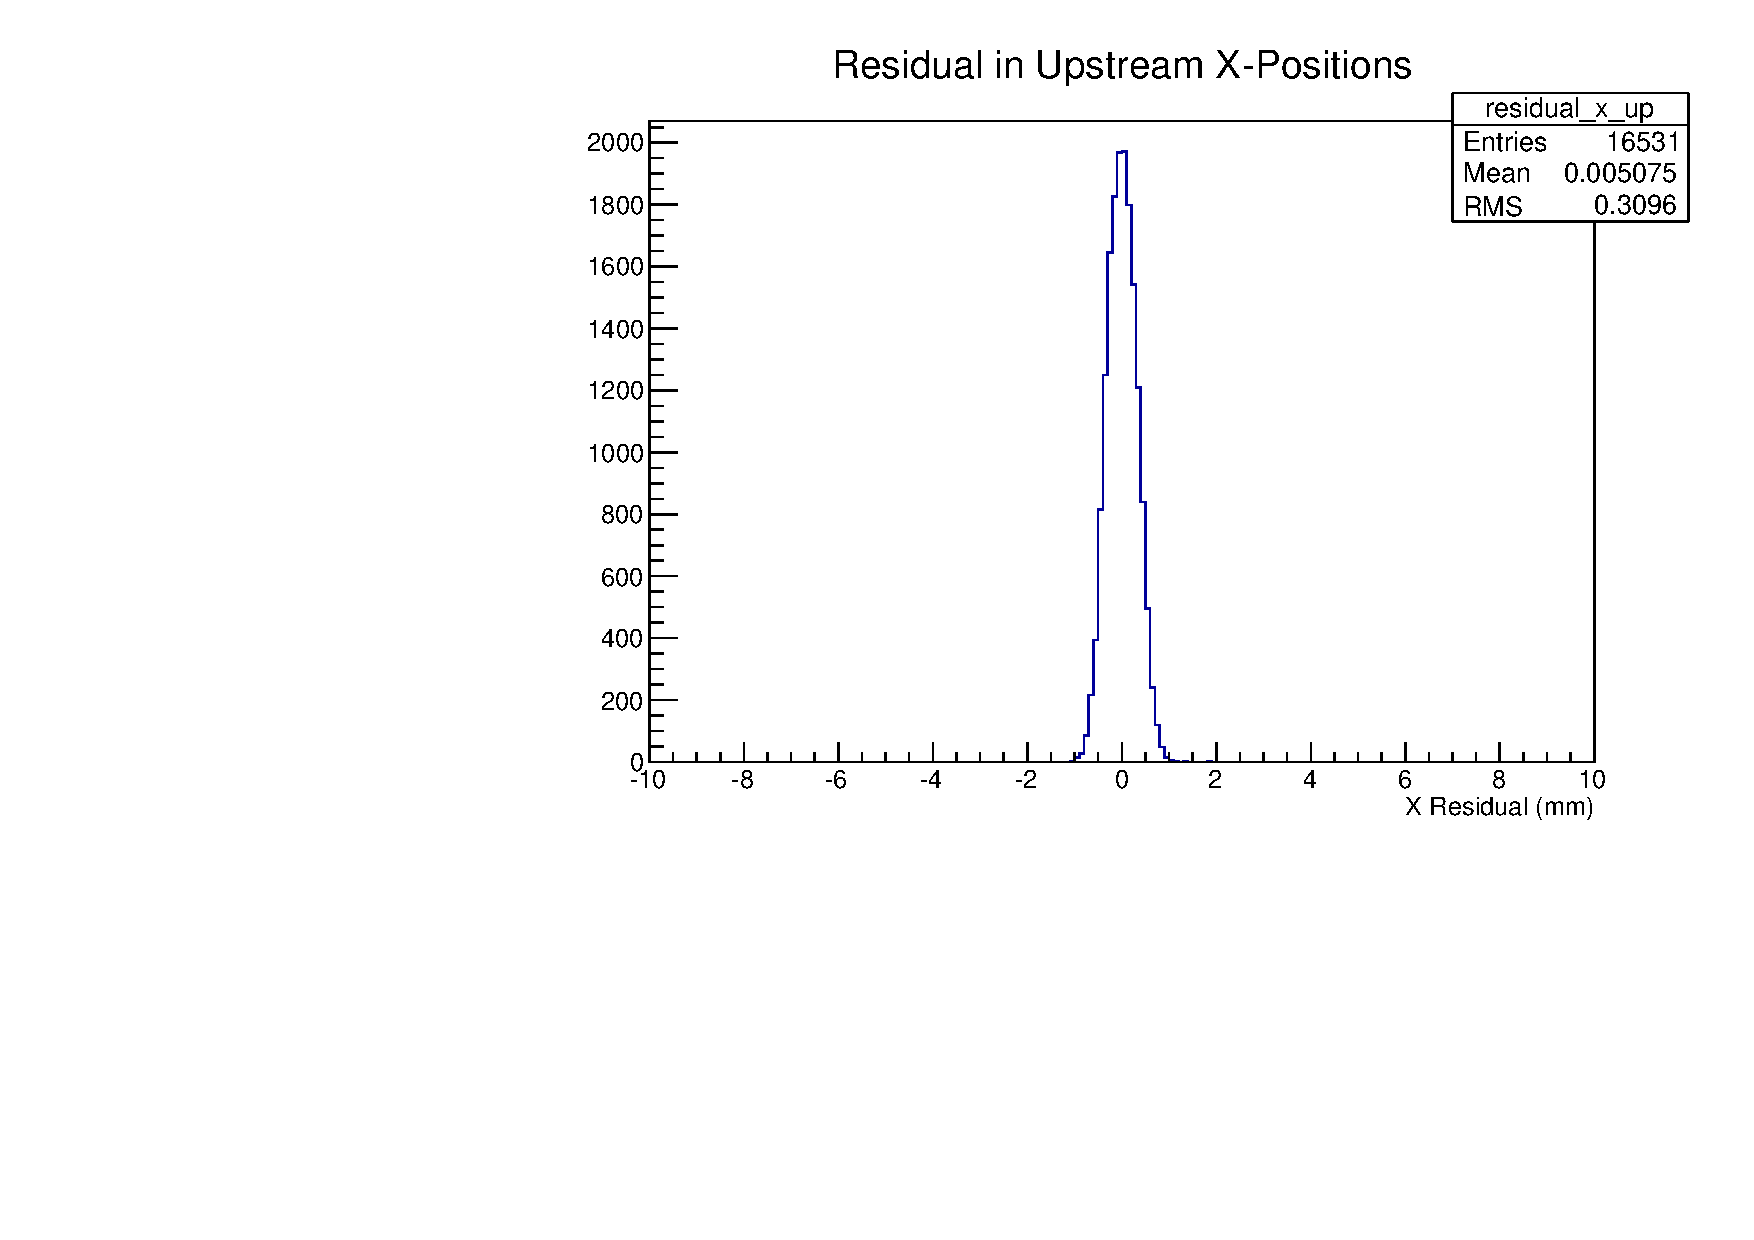
\includegraphics[width=0.49\textwidth, angle=0]{08-Performance/residual_x_up.pdf}
      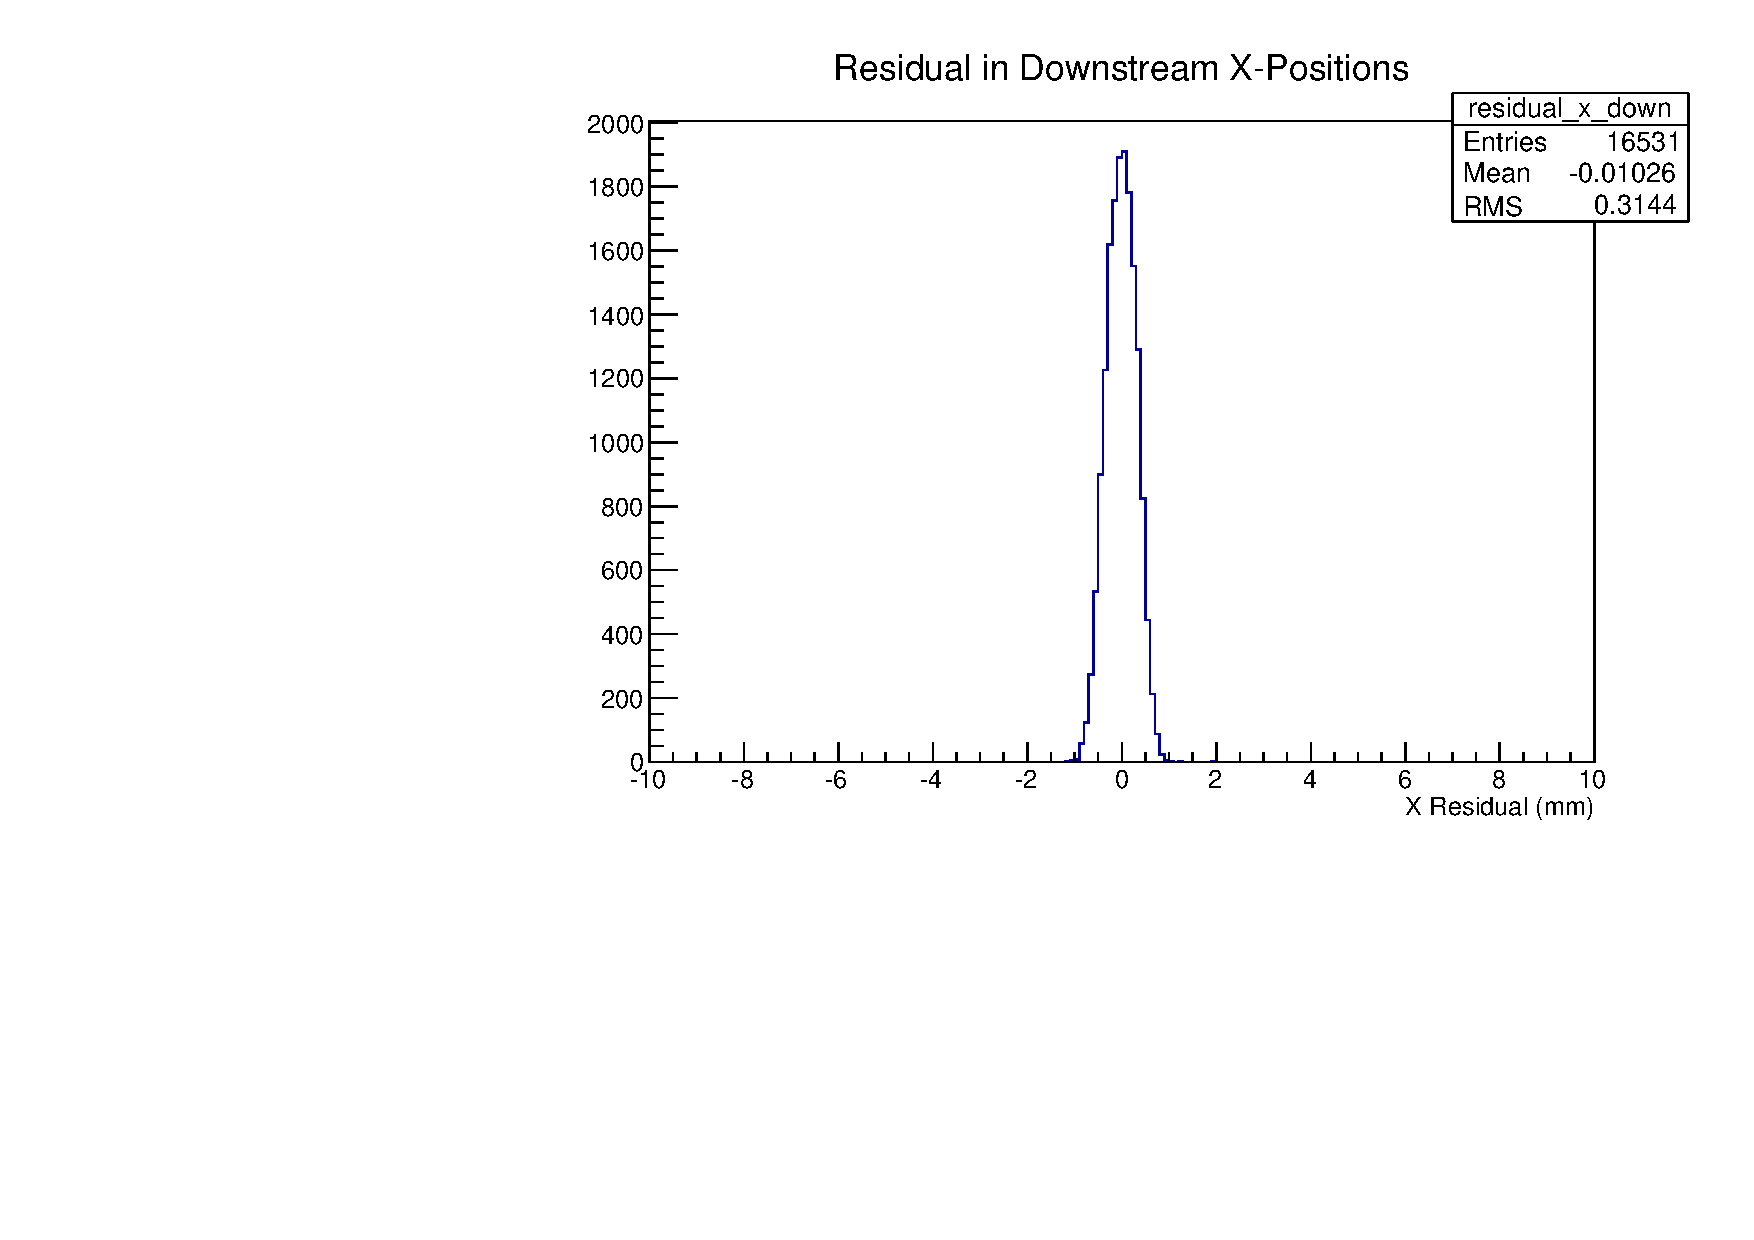
\includegraphics[width=0.49\textwidth, angle=0]{08-Performance/residual_x_down.pdf}
      \caption{\label{fig:XResidKalman} The $x$ residuals of the upstream (left) and downstream (right) trackers for a 6~mm 4D emittance, and 200~MeV/c momentum beam.}
    \end{center}
  \end{figure}
  
    \begin{figure}[p]
    \begin{center}
      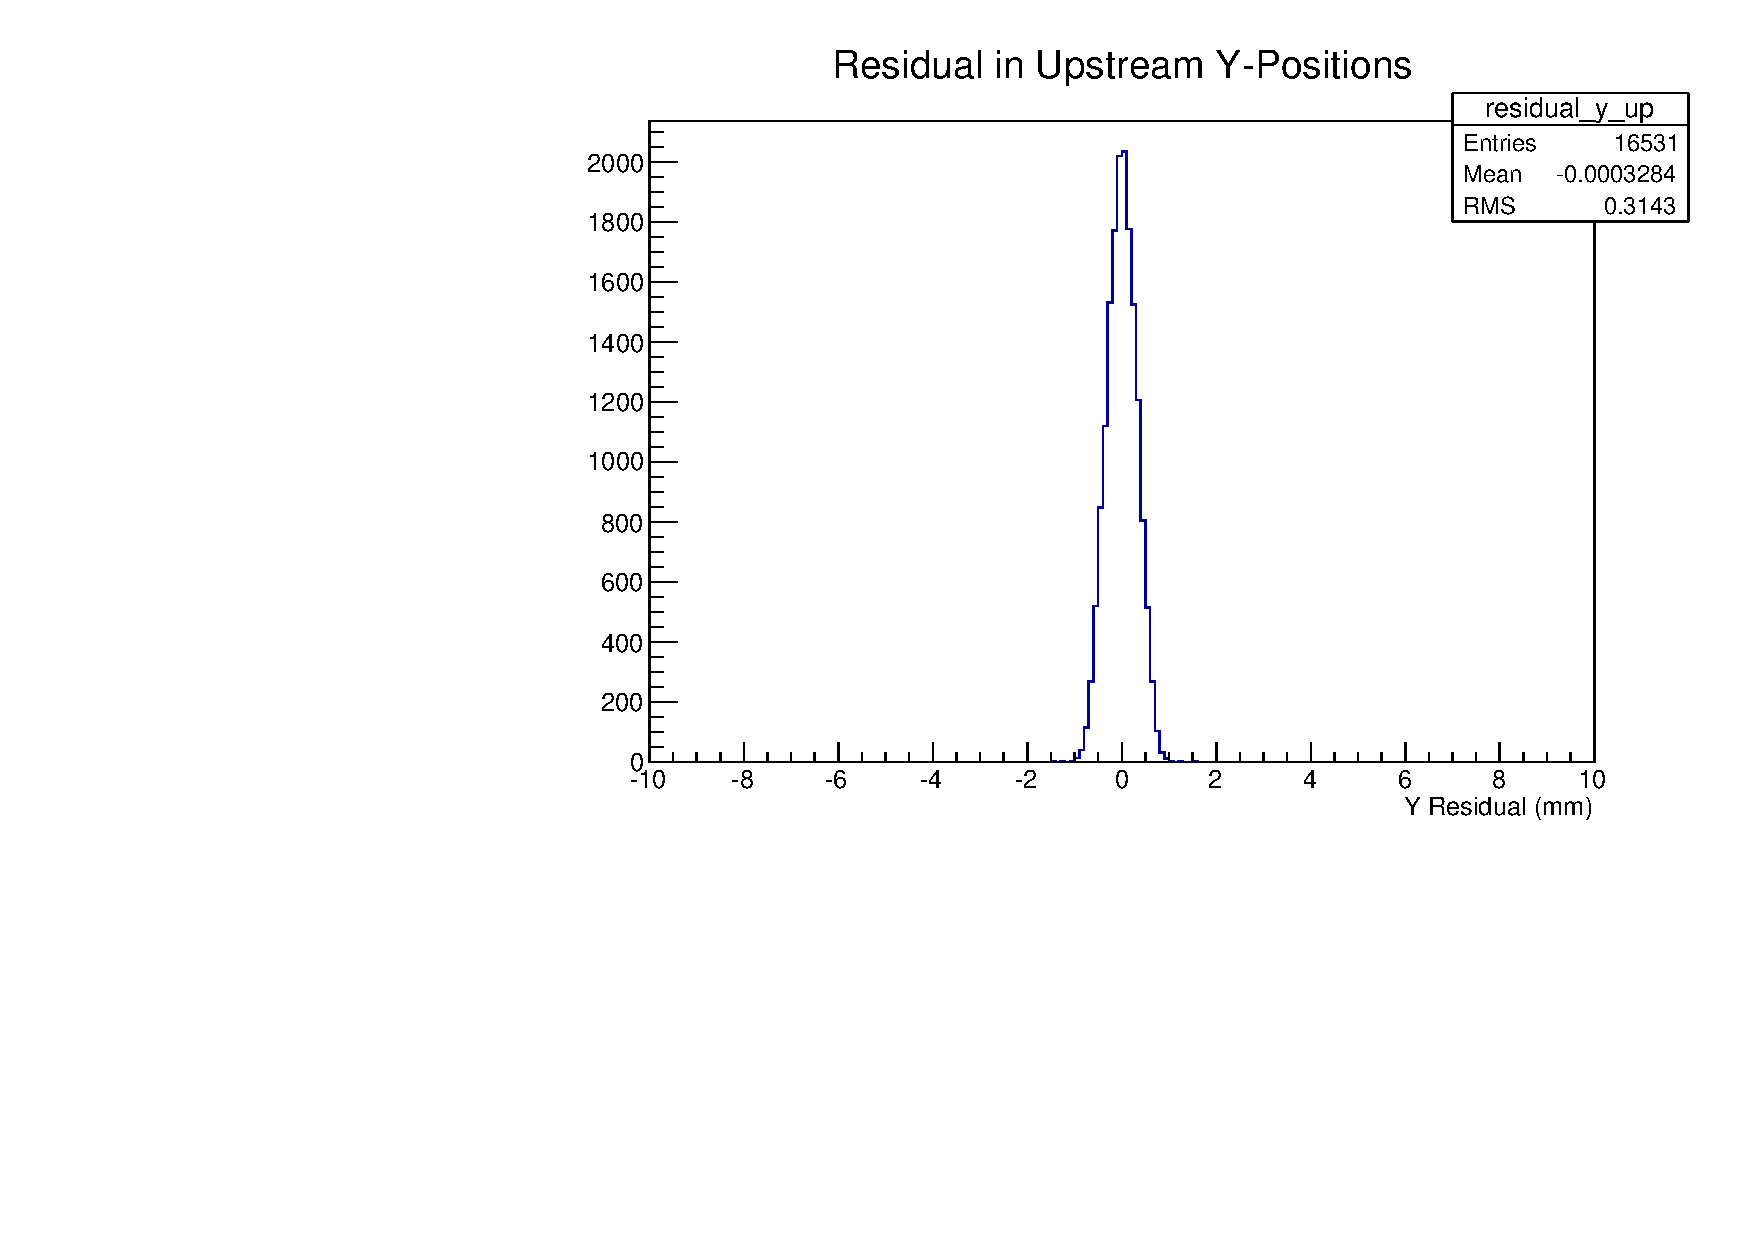
\includegraphics[width=0.49\textwidth, angle=0]{08-Performance/residual_y_up.pdf}
      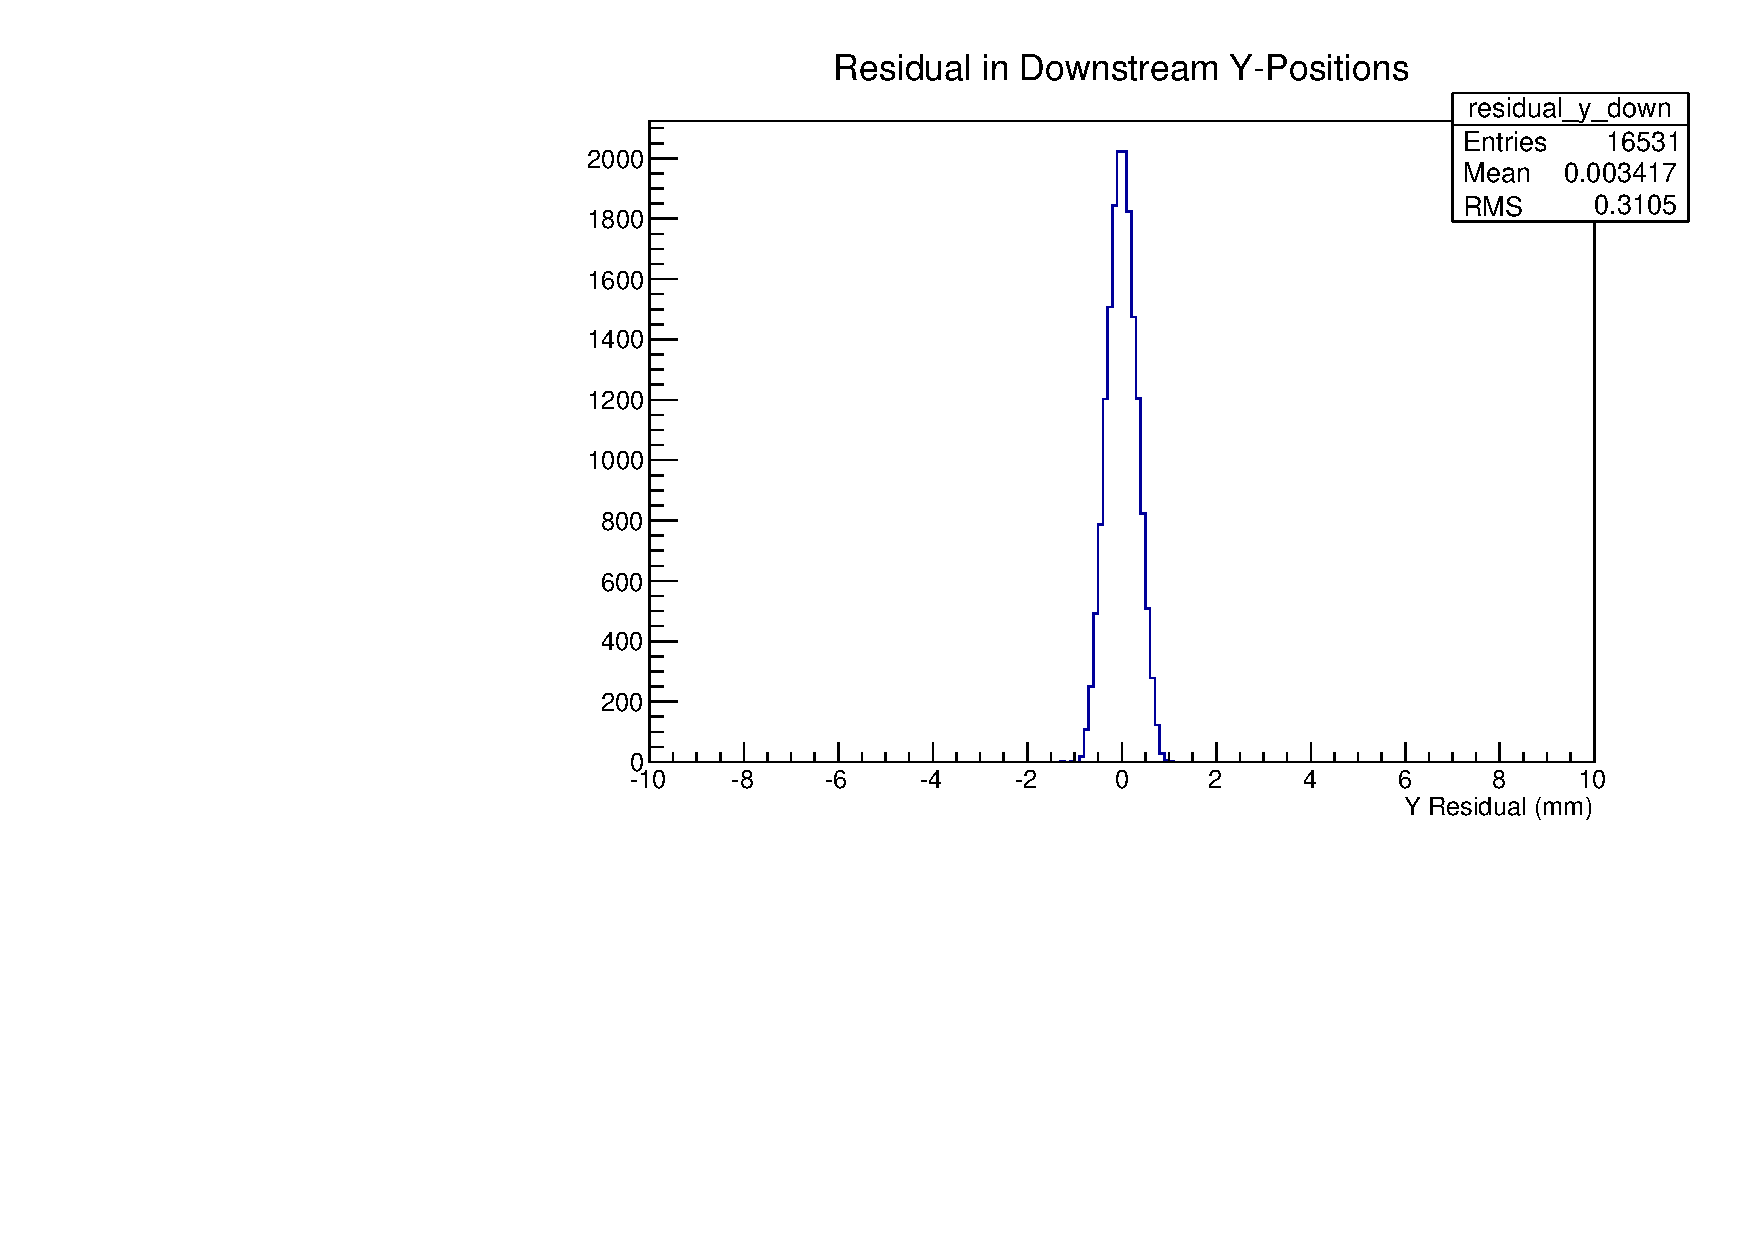
\includegraphics[width=0.49\textwidth, angle=0]{08-Performance/residual_y_down.pdf}
      \caption{\label{fig:YResidKalman} The $y$ residuals of the upstream (left) and downstream (right) trackers for a 6~mm 4D emittance, and 200~MeV/c momentum beam.}
    \end{center}
  \end{figure}
  
  
  \begin{figure}[p]
    \begin{center}
      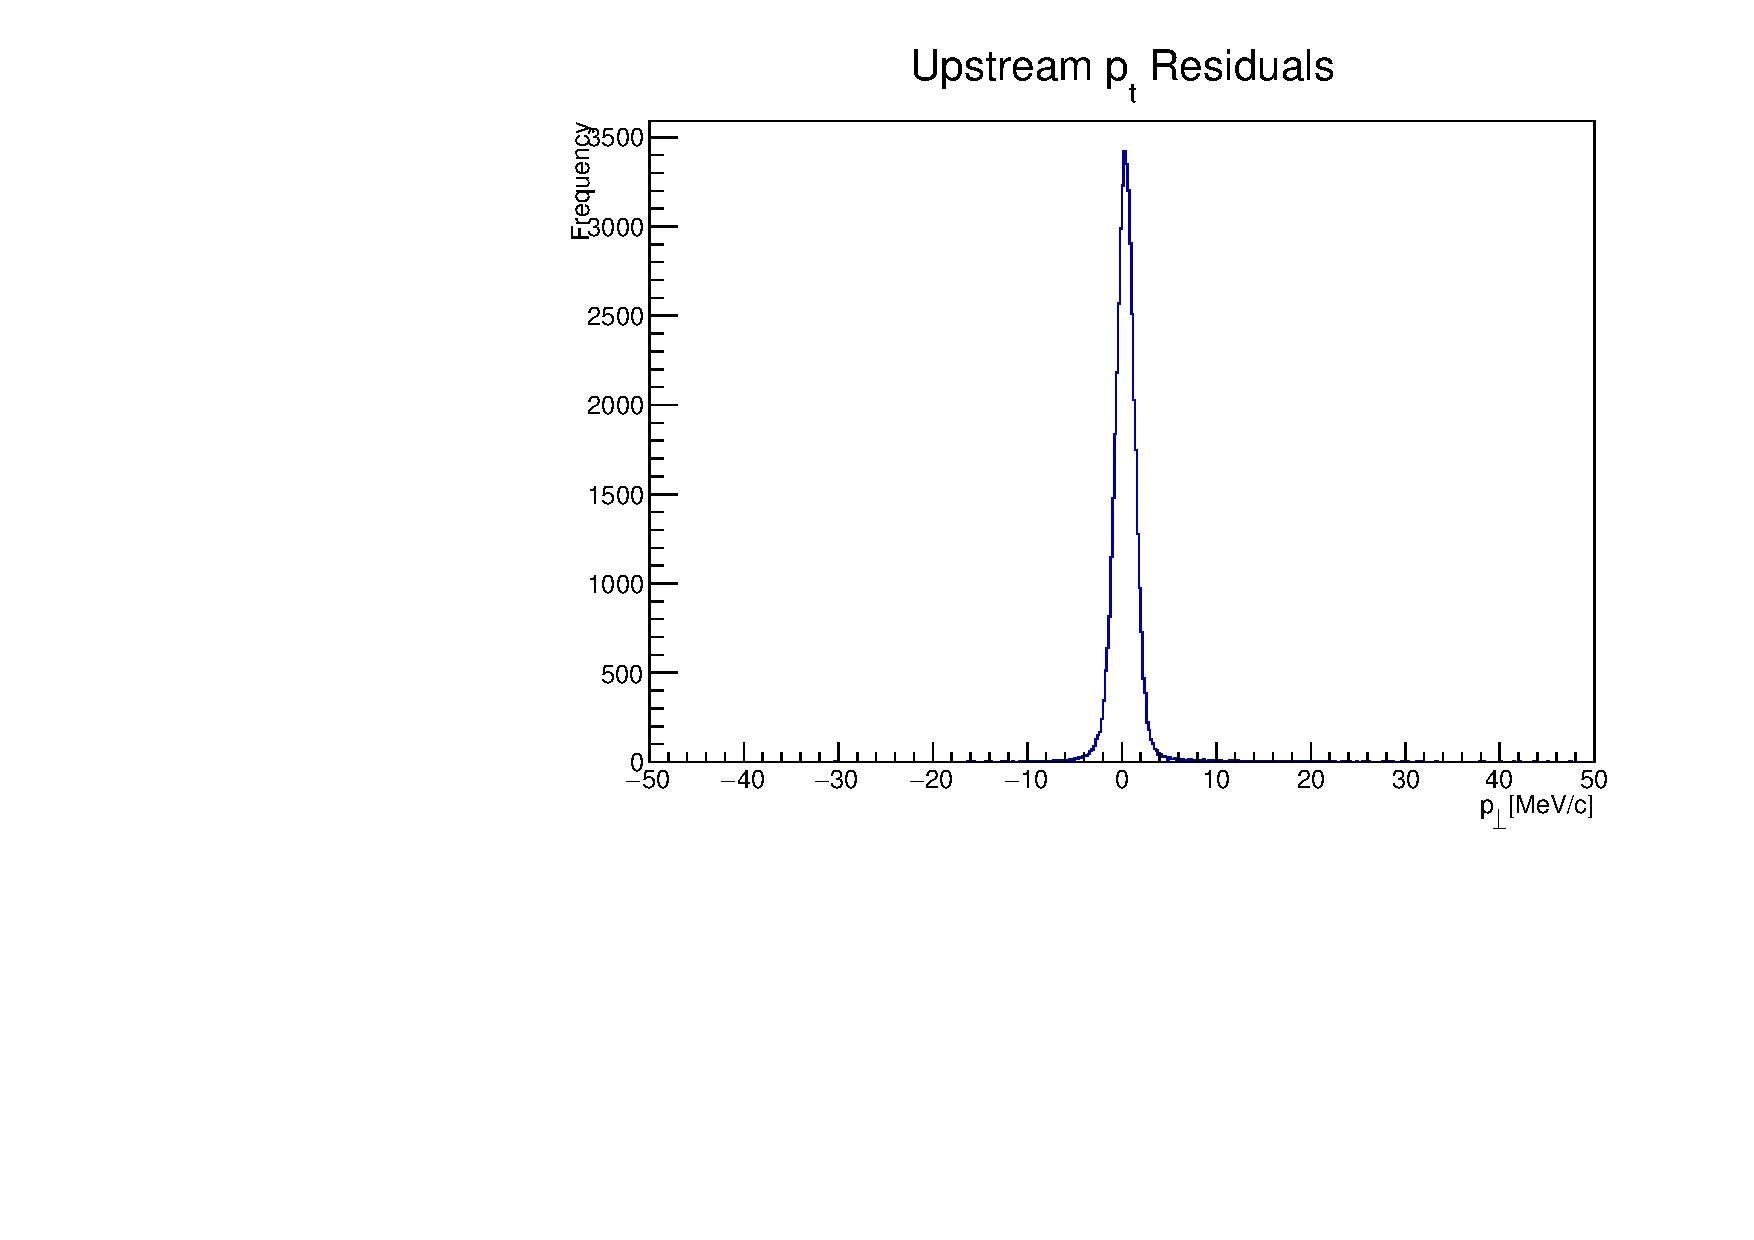
\includegraphics[width=0.49\textwidth, angle=0]{08-Performance/upstream_residual_pt.pdf}
      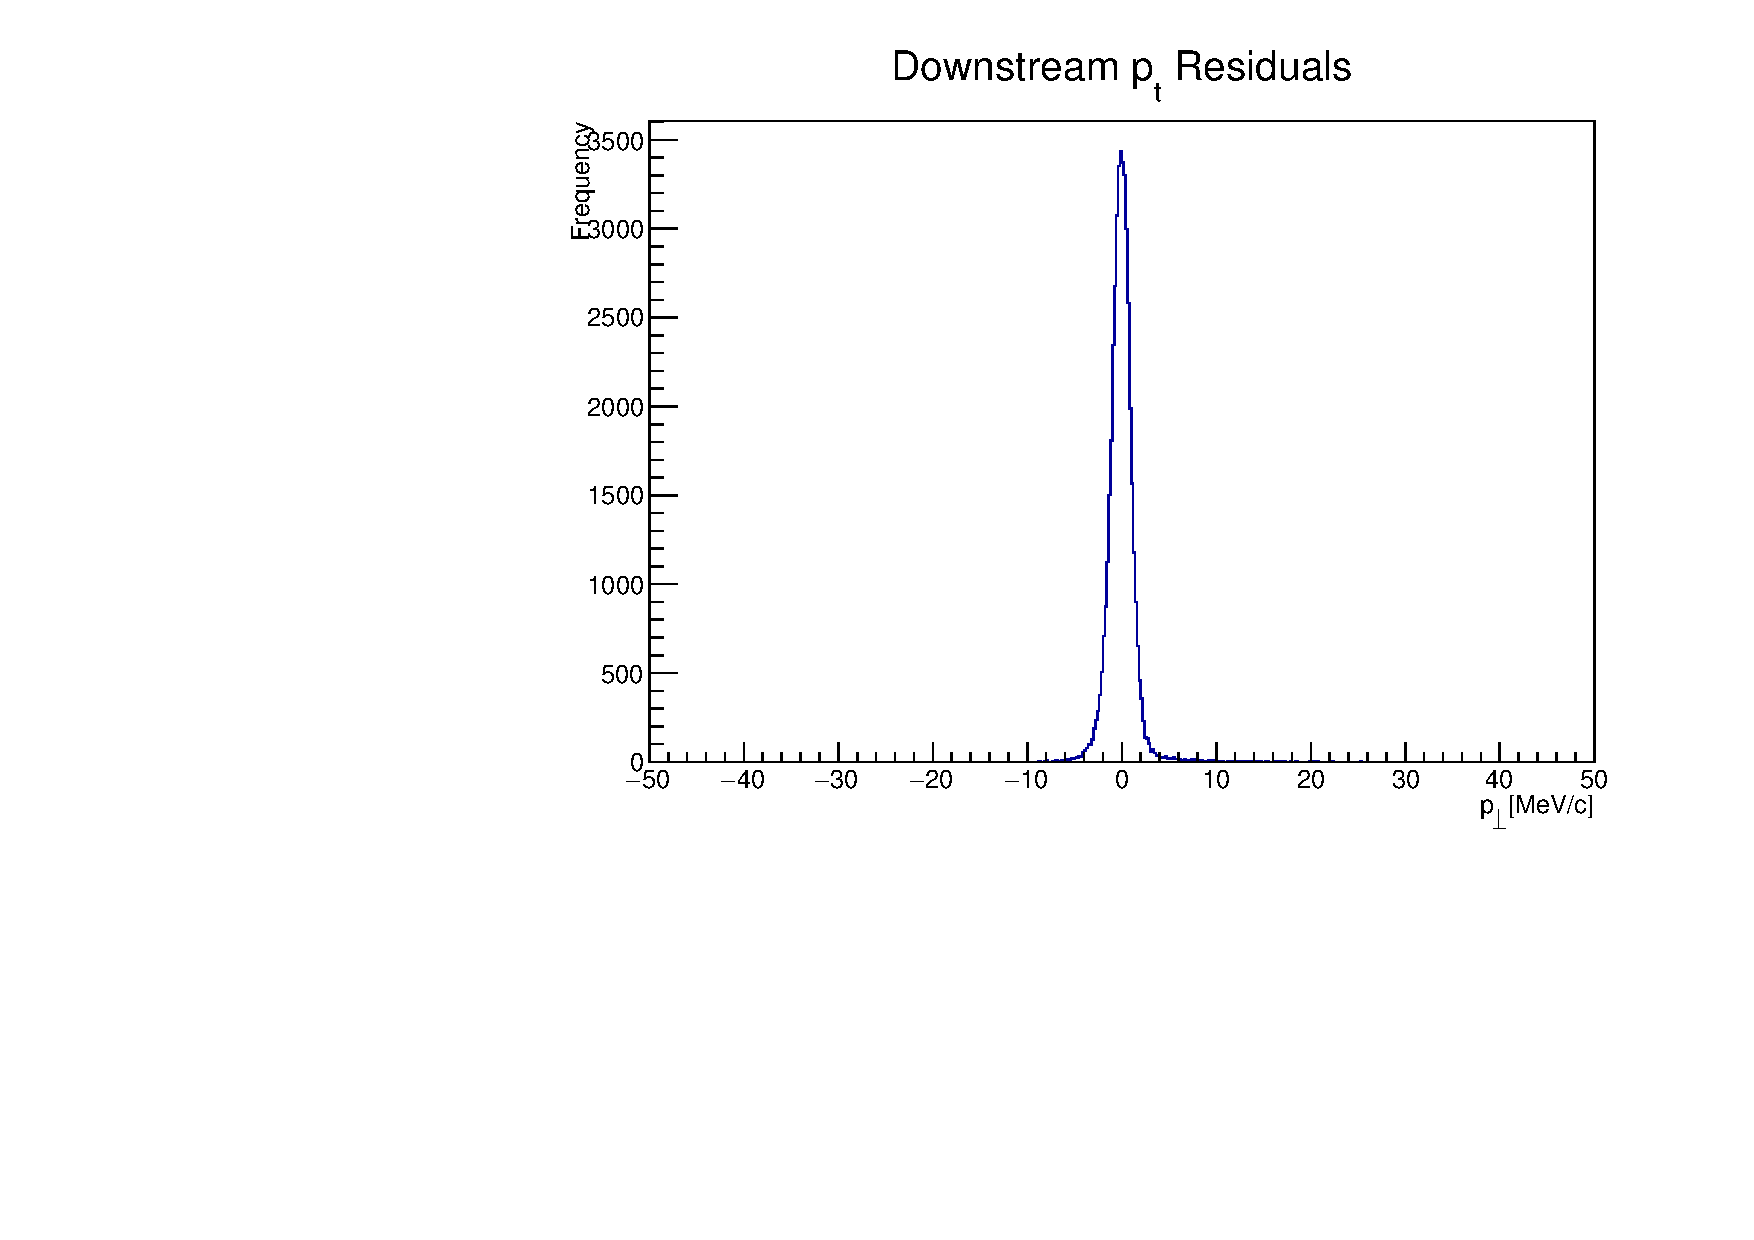
\includegraphics[width=0.49\textwidth, angle=0]{08-Performance/downstream_residual_pt.pdf}
      \caption{\label{fig:PtResidKalman} The $p_t$ residuals of the upstream (left) and downstream (right).}
    \end{center}
  \end{figure}
  
   \begin{figure}[p]
    \begin{center}
      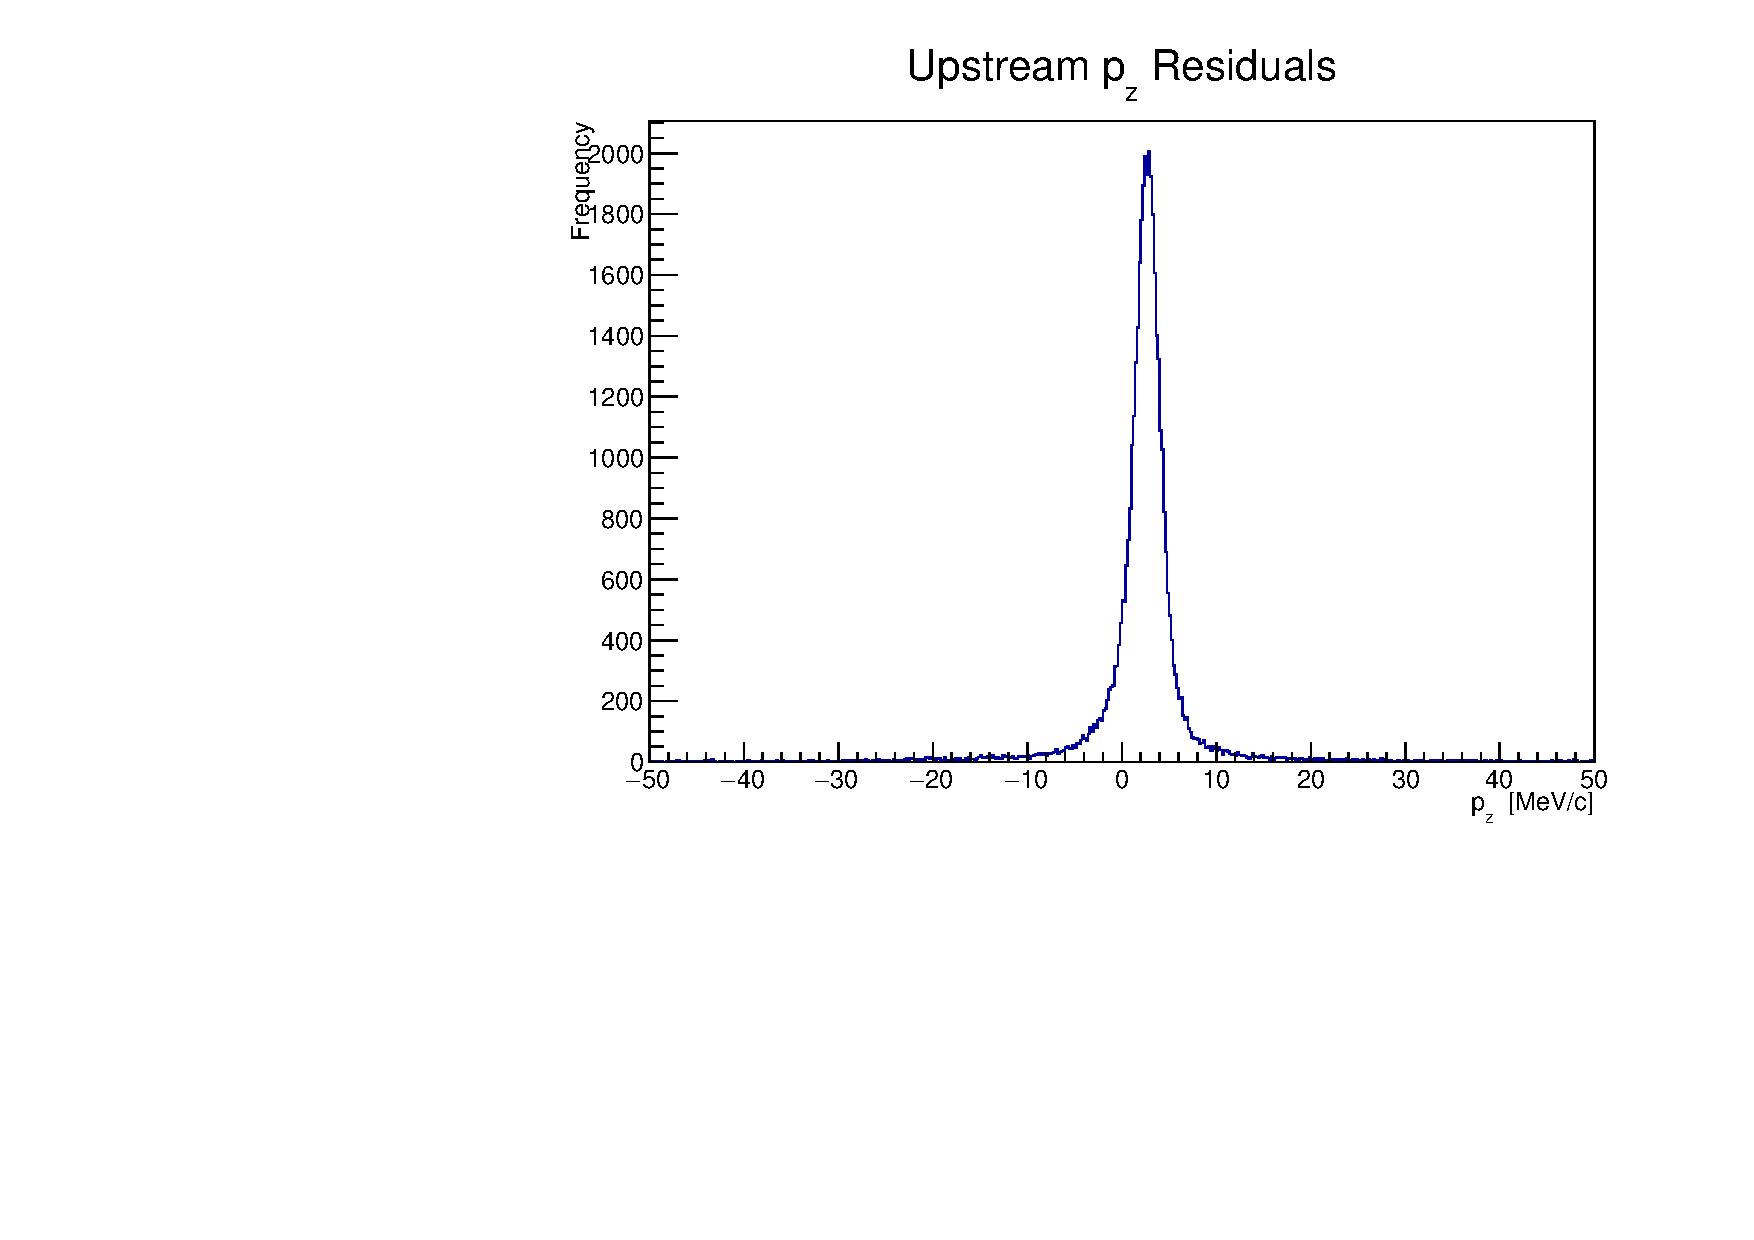
\includegraphics[width=0.49\textwidth, angle=0]{08-Performance/upstream_residual_pz.pdf}
      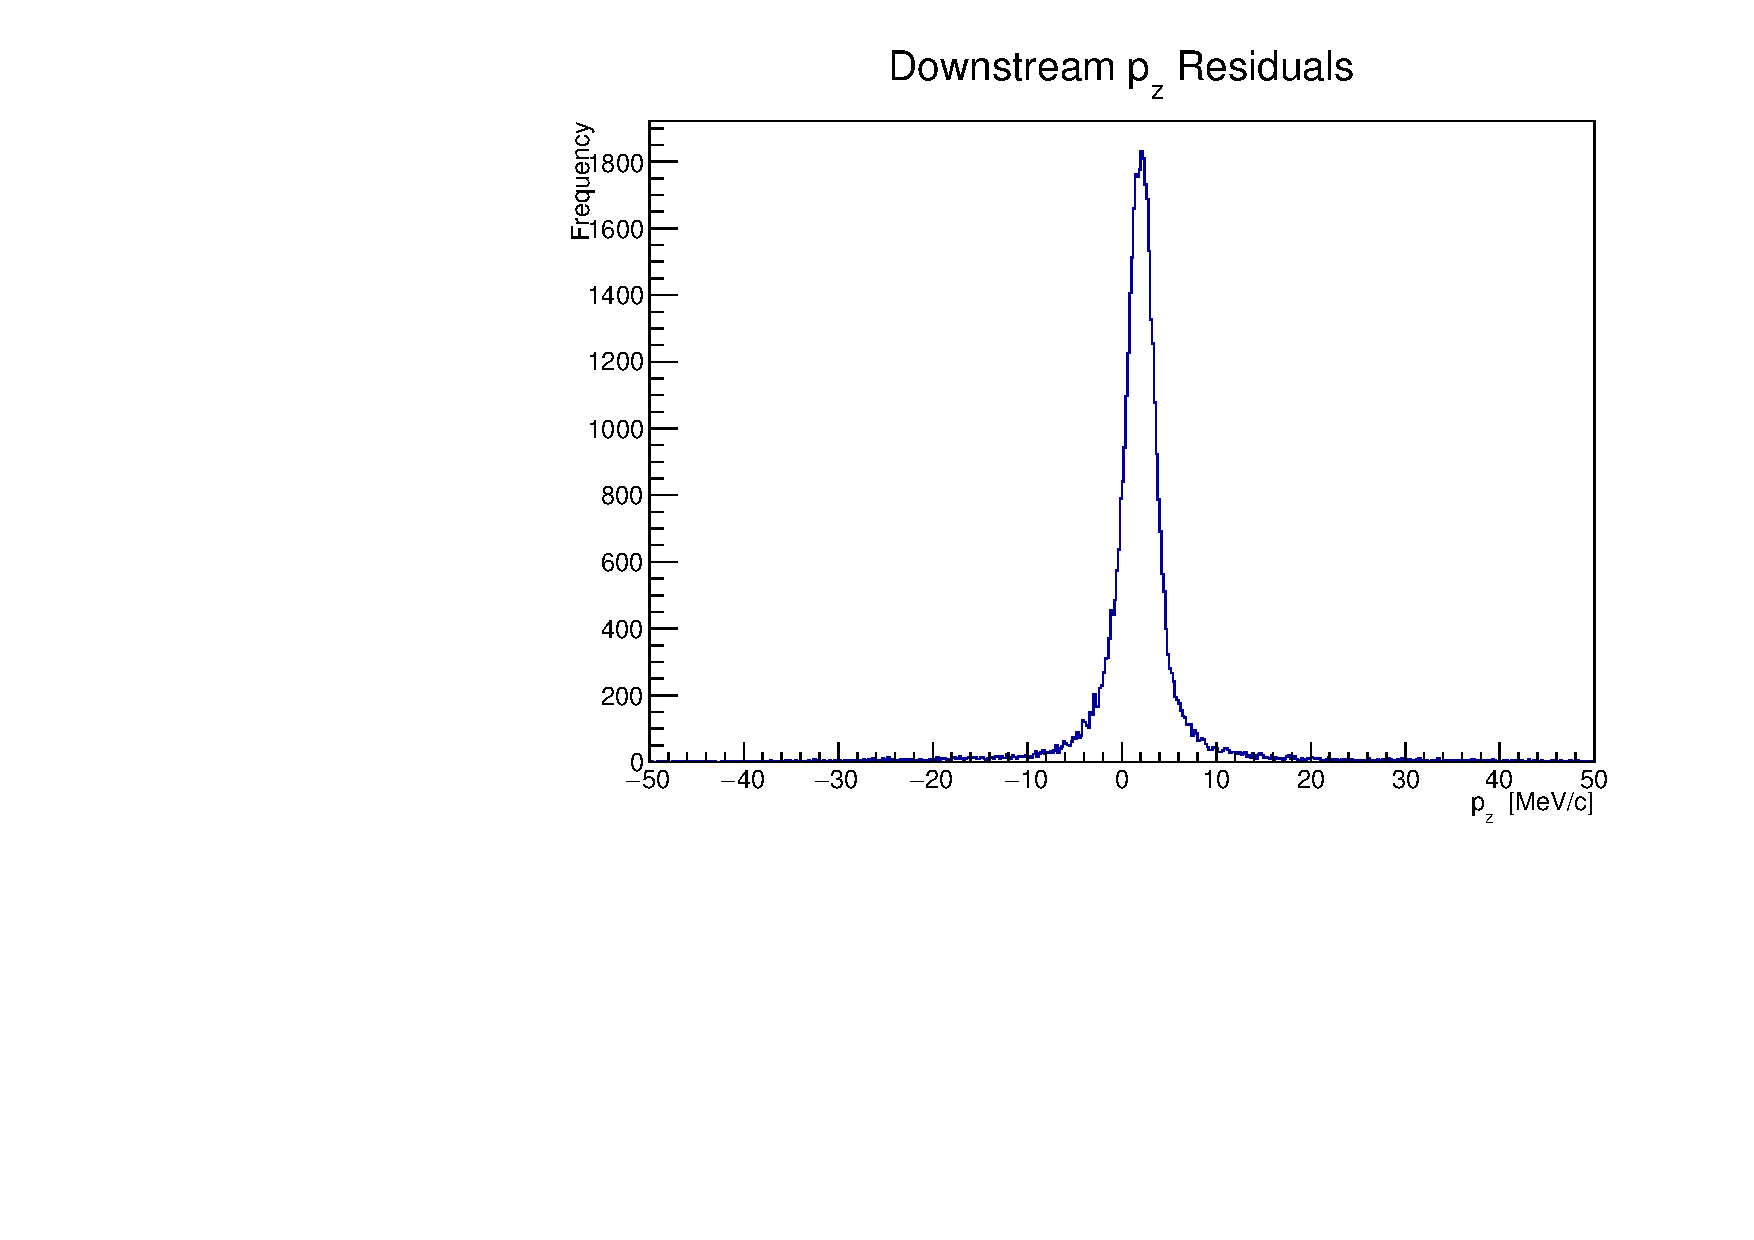
\includegraphics[width=0.49\textwidth, angle=0]{08-Performance/downstream_residual_pz.pdf}
      \caption{\label{fig:PzResidKalman} The $p_z$ residuals of the upstream (left) and downstream (right) trackers for a 6~mm 4D emittance, and 200~MeV/c momentum beam.}
    \end{center}
  \end{figure}
  
  \begin{figure}[p]
   \begin{center}
     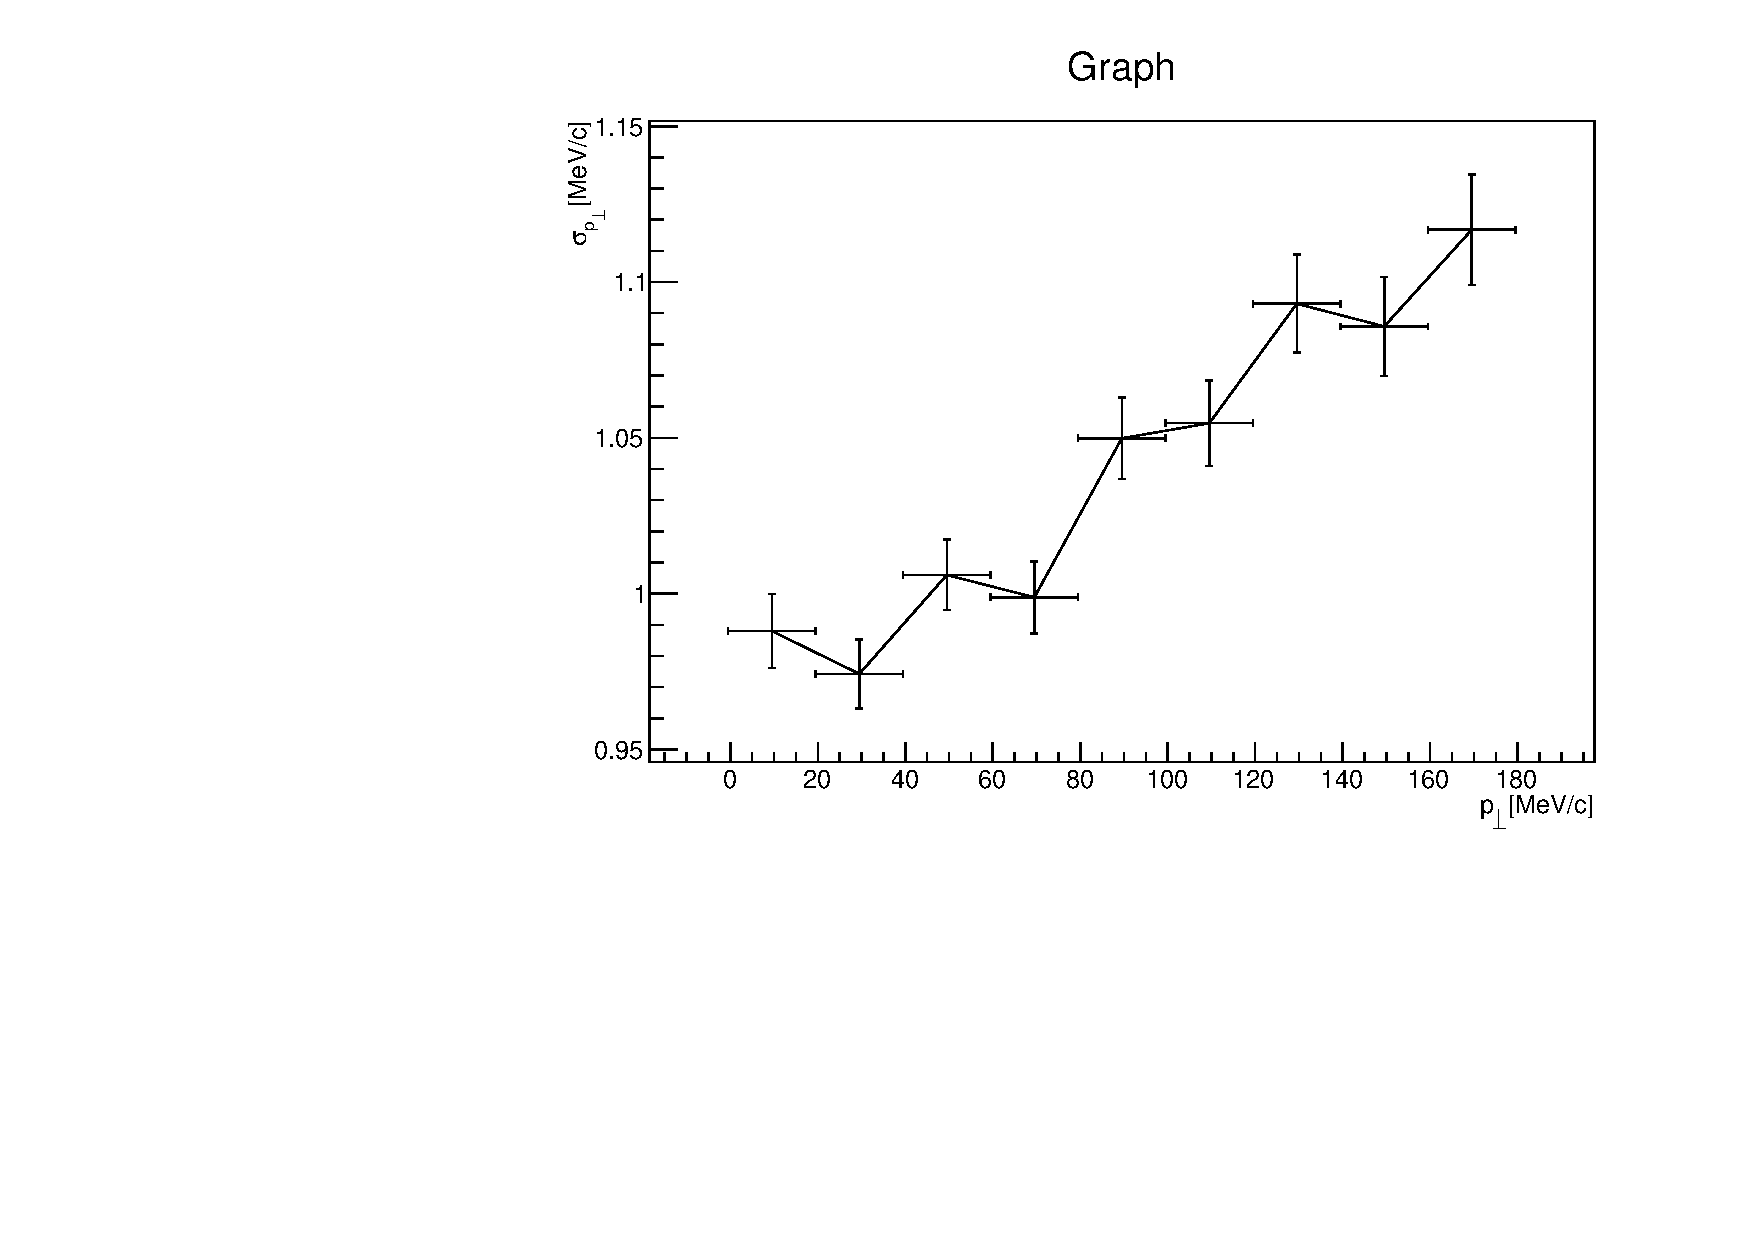
\includegraphics[width=0.49\textwidth, angle=0]{08-Performance/downstream_pt_resolution_vs_pt.pdf}
     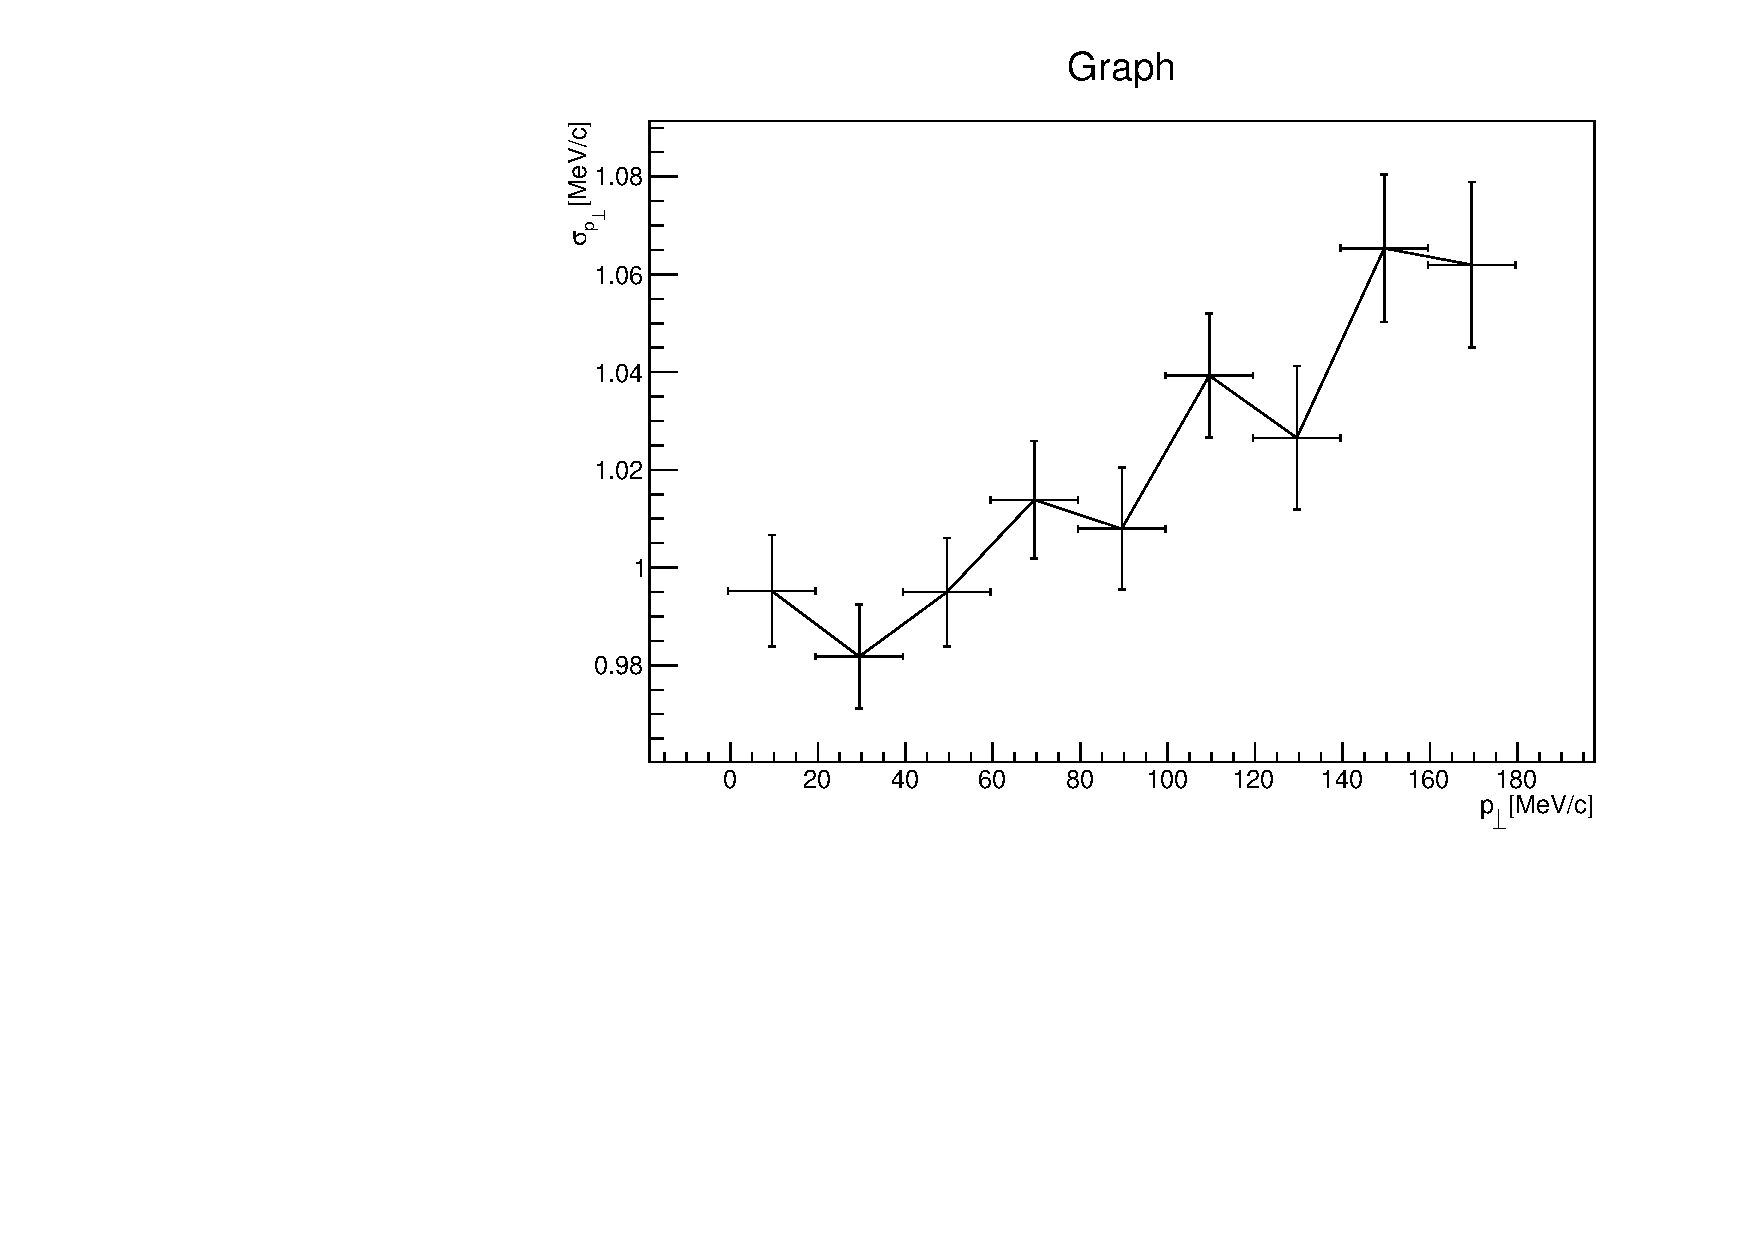
\includegraphics[width=0.49\textwidth, angle=0]{08-Performance/upstream_pt_resolution_vs_pt.pdf}
     \caption{\label{fig:PtPtResolKalman} The $p_t$ resolution vs the $p_t$ of the upstream (left) and downstream (right).}
   \end{center}
  \end{figure}
  
  \begin{figure}[p]
   \begin{center}
     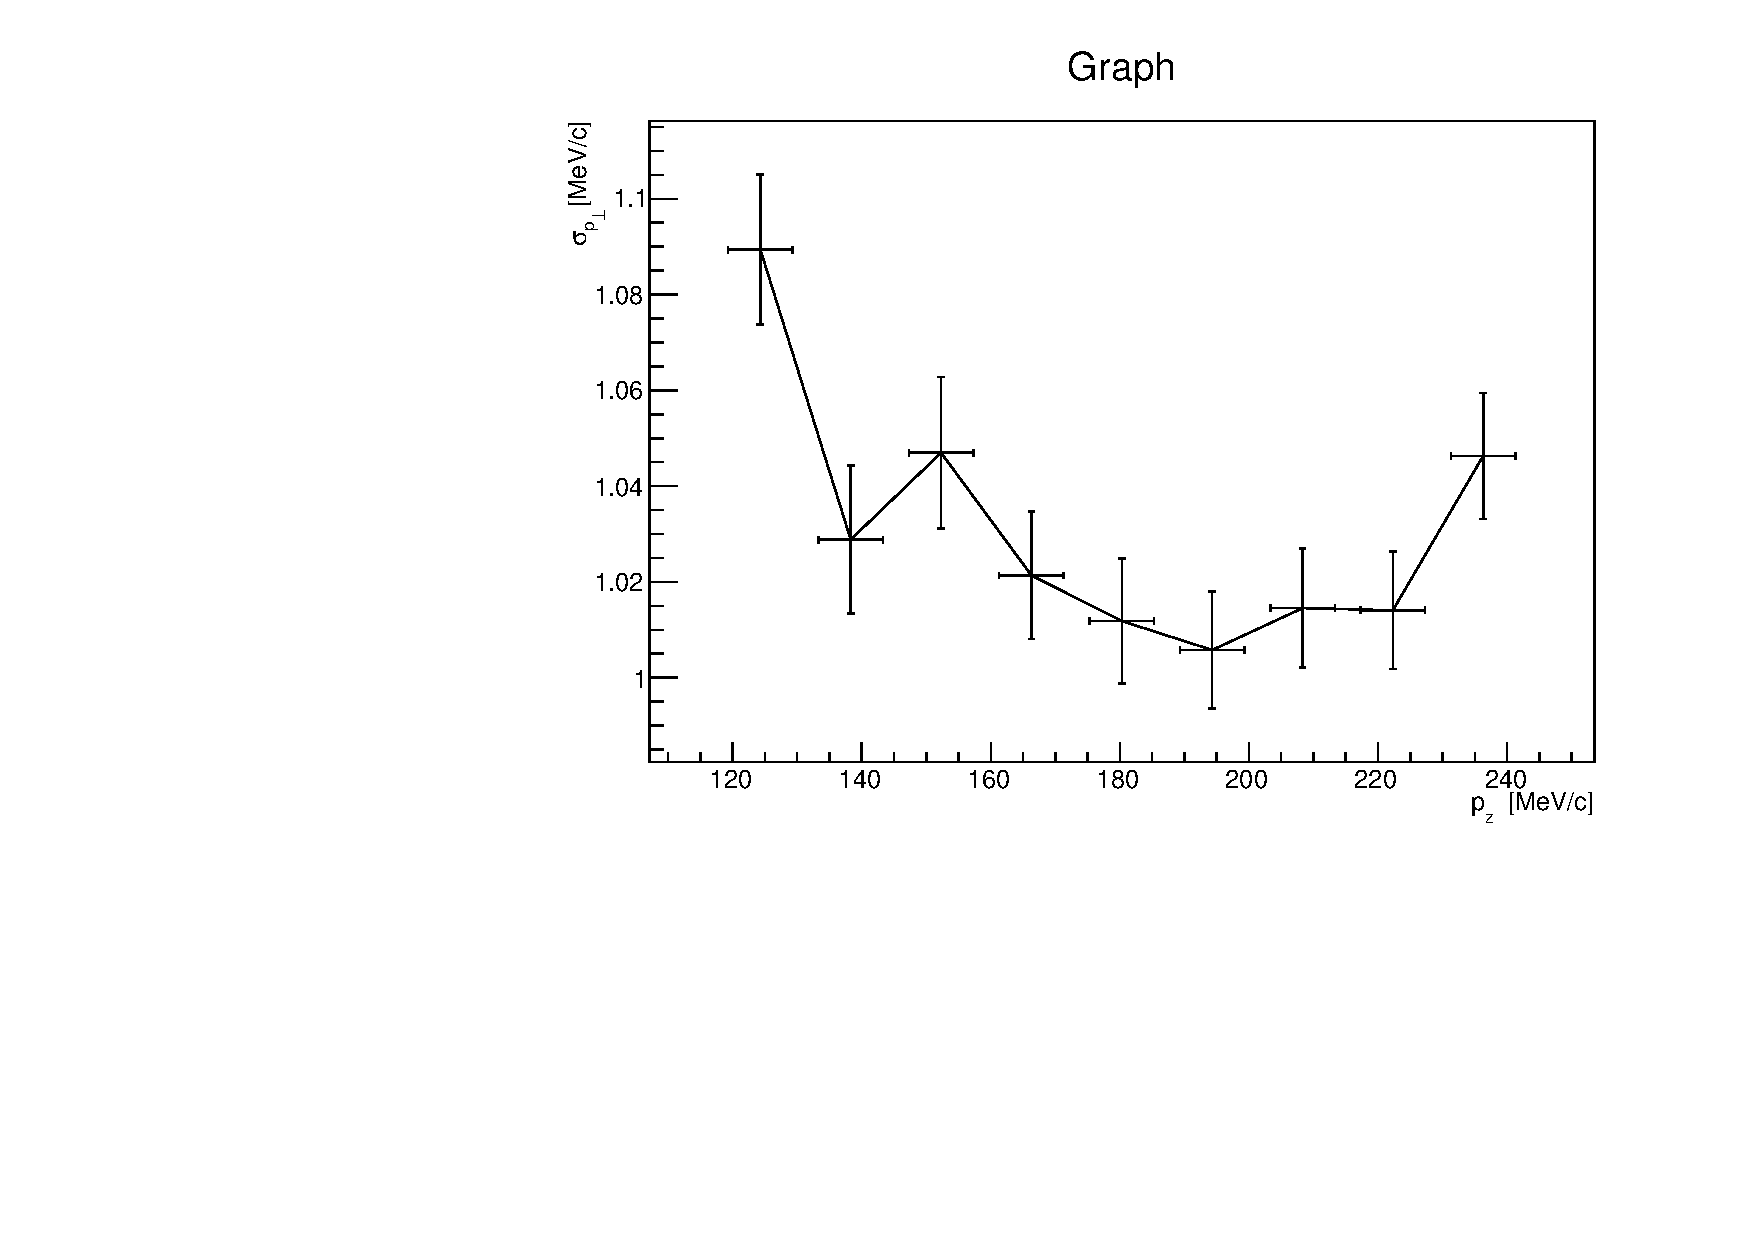
\includegraphics[width=0.49\textwidth, angle=0]{08-Performance/downstream_pz_resolution_vs_pt.pdf}
     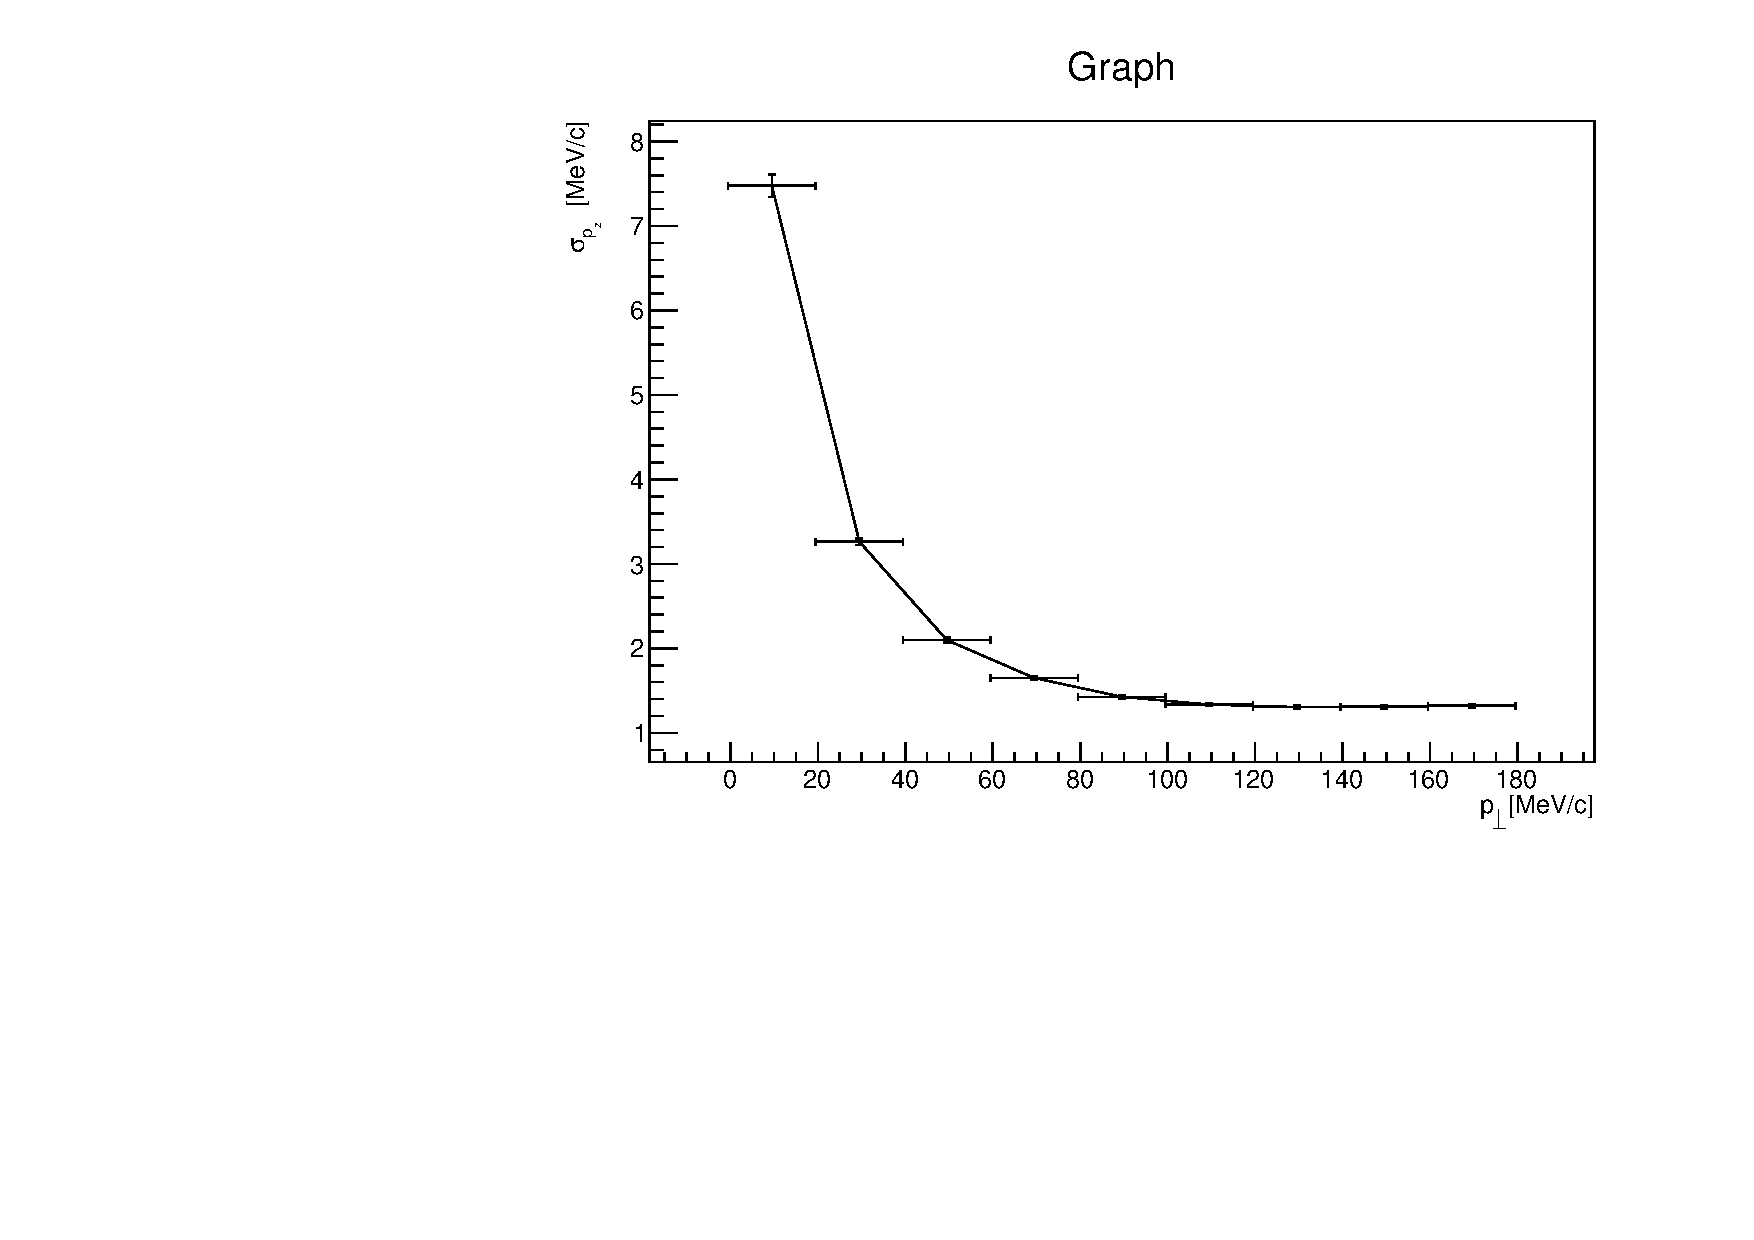
\includegraphics[width=0.49\textwidth, angle=0]{08-Performance/upstream_pz_resolution_vs_pt.pdf}
     \caption{\label{fig:PtPzResolKalman} The $p_z$ resolution vs the $p_t$ of the upstream (left) and downstream (right).}
   \end{center}
  \end{figure}